\section{Buffer Amplifier}

Figure 3 shows the schematic of the Buffer amplifieri.

\begin{figure}[h!]
  \centering
  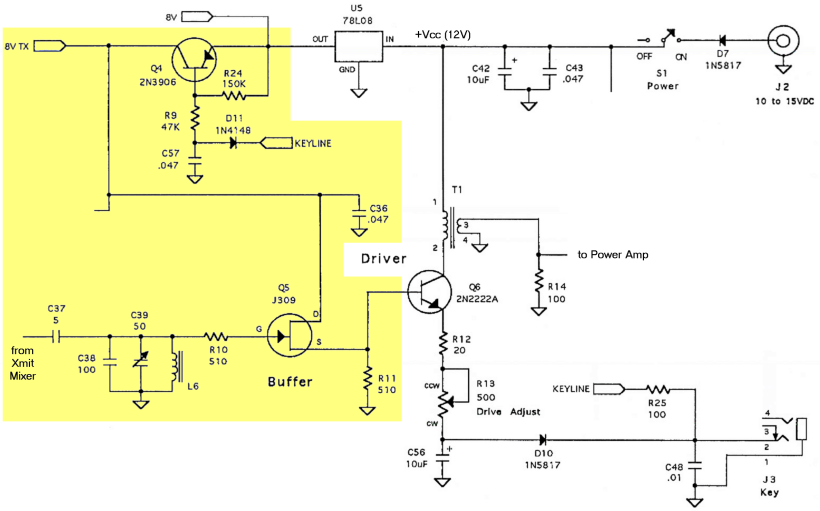
\includegraphics[scale=0.5]{./img/BuffAmp.png}
  \label{BuffAmp}
  \caption{Circuit Schematic for the Buffer Amplifier}
\end{figure}

Such a circuit is a source-follower, and therefore has no impedance gain and a
high input impedance. The function generator was connected to $C_{37}$ with
the $1.5k\Omega$ resistor. The frequency used was $7.04V$ and the amplitude was $1V_{pp}$.

\subsection{Max Voltage Across \bm{$R_{10}$}}
$C_{39}$ was adjusted for maximum voltage. The measured maximum value
was $\boxed{65.1 V_{RMS}}$.

\subsection{Voltage Gain \bm{$G_v$} across \bm{$R_{11}$}}
The voltage gain across $R_{11}$ was calculated to be:
\begin{align*}
  G_v &= 20log\bigg( \frac{v}{v_i} \bigg)
      \implies 20log\bigg( \frac{1.09V}{65.1mV} \bigg)
      = \boxed{24.5 \text{dB}}
\end{align*}


\subsection{Power Gain, \bm{$G_P$}}
Given that a $1.5k\Omega$ resistor is at the input and a $510\Omega$ is
at the load, the power gain was calculated to be:
\begin{align*}
  G_P &= 10log\bigg( \frac{P}{P_0} \bigg)
      \implies 10log\bigg( \frac{2.33mW}{2.83\mu W} \bigg)
      = \boxed{29.2 \text{dB}}
\end{align*}


